\chapter{Вклад}
\label{chap:impl}

Мы предлагаем новый подход к гетерогенному планированию. Он основан на обходе графов переходов состояний выполняемых программ, который изображён на рис.~\ref{fig:jSTGExample}. Более конкретно, наш вклад заключается в следующем:
%
\begin{itemize}
\item Теоретически оптимальный гетерогенный планировщик. В отличие от других существующих планировщиков, наш учитывает не только время отклика программ, но и потребление энергии;
\item Эвристика планирования, которая позволяет принимать решения о планировании значительно быстрее, чем оптимальный планировщик. Мы также демонстрируем, что некоторые эвристики близки к оптимальным;
\item Прототип инструмента на C++, реализующего все наши планировщики;
\item Подробное сравнение всех предложенных планировщиков.
\end{itemize}
%

\section{Ограничения}
На данный момент наши планировщики не учитывают накладные расходы на преемственность и миграцию. Однако предложенная методология графов переходов состояний легко расширяется до таких более реалистичных сценариев.

\begin{figure*}
\center
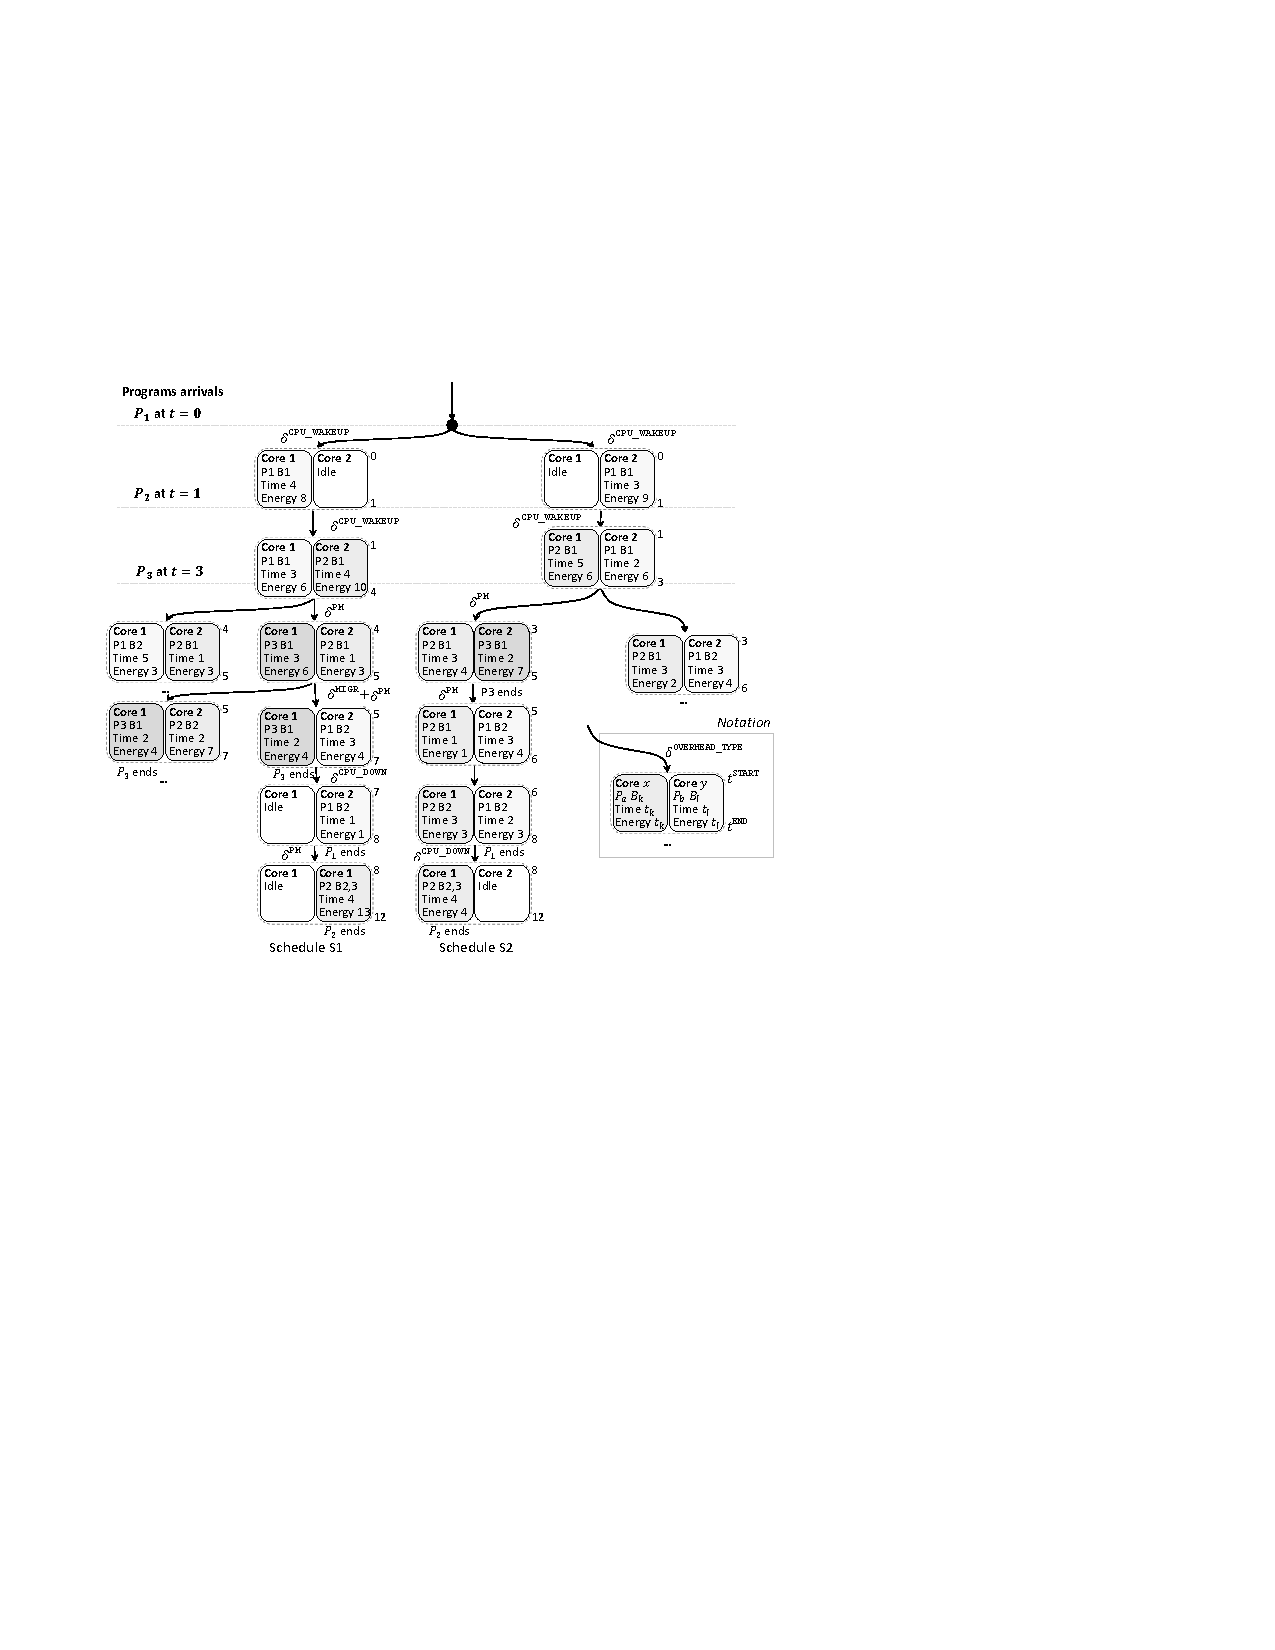
\includegraphics[width=.9\textwidth]{figs/jSTG.pdf}
\caption{Объединённый граф программ с расписаниями из рис.~\ref{fig:twoSchedulesExample}. Случай безпреемственного планирования}
\label{fig:jSTGExample}
\end{figure*}